\documentclass[12pt,twoside,letterpaper]{article}
\usepackage{booktabs}
\newcommand{\reporttitle}{Project: Werewolf On-Chain Game}
\newcommand{\reportauthorTwo}{}
\newcommand{\cidTwo}{A0319170J}
\newcommand{\reportauthorThree}{}
\newcommand{\cidThree}{A0318793N}
\newcommand{\reportauthorFour}{}
\newcommand{\cidFour}{A0326802J}

\newcommand{\reporttype}{Coursework}
\bibliographystyle{plain}

\input{includes}
\input{notation}

\begin{document}

\input{titlepage}



\section{Behavior}

\subsection{Algorithm Examination}

\subsubsection{Finite State Machine Structure}

The behavior node coordinates the drone's mission using a seven-state FSM. Table~\ref{tab:fsm_states} summarises the states, their waypoints, and the conditions under which they transition.

\begin{table}[htbp]
    \centering
    \caption{FSM states, waypoints, and transition conditions.}
    \label{tab:fsm_states}
    \vspace{0.1cm}
    \begin{tabular}{llll}
        \toprule
        \textbf{State} & \textbf{Waypoint} & \textbf{Transition condition} & \textbf{Next state} \\
        \midrule
        \textsc{Begin}    & ---                             & On startup                  & \textsc{Takeoff} \\
        \textsc{Takeoff}  & $(x_0,\, y_0,\, h_c)$          & Reached \& turtle stopped   & \textsc{Initial} \\
                          &                                 & Reached \& turtle running   & \textsc{Turtle\_Position} \\
        \textsc{Turtle\_Position} & turtle position at $h_c$ & Reached               & \textsc{Turtle\_Waypoint} \\
        \textsc{Turtle\_Waypoint} & turtle goal at $h_c$     & Reached               & \textsc{Initial} \\
        \textsc{Initial}  & $(x_0,\, y_0,\, h_c)$          & Reached \& turtle stopped   & \textsc{Landing} \\
                          &                                 & Reached \& turtle running   & \textsc{Turtle\_Position} \\
        \textsc{Landing}  & $(x_0,\, y_0,\, z_0)$          & Reached                     & \textsc{End} \\
        \textsc{End}      & ---                             & Motors off, timer cancelled & --- \\
        \bottomrule
    \end{tabular}
\end{table}

The drone repeats the three-step cycle \textsc{Turtle\_Position} $\to$ \textsc{Turtle\_Waypoint} $\to$ \textsc{Initial} until the turtlebot stops. The \texttt{turtle\_stop\_} flag is checked only at \textsc{Initial} (and \textsc{Takeoff}), so the cycle always finishes before the landing decision is made.

\subsubsection{Waypoint Reaching}

A waypoint is reached when the 3D Euclidean distance drops below the threshold $r_{\text{thres}}$:
\[
    d = \sqrt{(\Delta x)^2 + (\Delta y)^2 + (\Delta z)^2} < r_{\text{thres}}
\]
Using the full 3D distance rather than 2D prevents the drone from triggering arrival while it is still climbing or descending toward the target altitude.

\subsection{Improvements}

\subsubsection{Live Waypoint Tracking for \textsc{Turtle\_Position}}

The template sets the waypoint once at the moment of state entry. The turtlebot moves at up to $0.22\,\text{m/s}$; at a behavior timer frequency of $10\,\text{Hz}$, it travels roughly $0.022\,\text{m}$ per tick. Over the several seconds the drone takes to fly to the turtle, the turtlebot can displace by $0.5$--$1\,\text{m}$. Chasing a stale waypoint causes the drone to land in empty space and immediately transition to \textsc{Turtle\_Waypoint}, skipping the actual interception.

The fix updates the waypoint on every timer tick while in \textsc{Turtle\_Position}:
\begin{verbatim}
if (state_ == TURTLE_POSITION && !turtle_plan_.poses.empty())
{
    waypoint_x_ = turtle_plan_.poses.front().pose.position.x;
    waypoint_y_ = turtle_plan_.poses.front().pose.position.y;
    waypoint_z_ = cruise_height_;
}
\end{verbatim}
The plan request that follows in the same tick then generates a fresh path to the updated target, keeping the controller on course.

\subsubsection{Cycle-Completion Guarantee}

If \texttt{turtle\_stop\_} were checked at every state, the drone could abort mid-cycle (e.g.\ during \textsc{Turtle\_Waypoint}) and attempt to land from an arbitrary position. Instead, the flag is evaluated only at \textsc{Initial} and \textsc{Takeoff}. This guarantees the drone completes the current visit before landing, matching the mission requirement that the cycle must complete.

An additional edge case arises if the turtlebot stops before the drone finishes taking off. In this case the drone transitions \textsc{Takeoff} $\to$ \textsc{Initial} $\to$ \textsc{Landing}, skipping the cycle entirely rather than performing a vacuous visit to a stationary turtle.

\subsubsection{Path Availability Guard}

\textsc{Turtle\_Plan\_} is populated only once the turtlebot begins moving. Both \textsc{Turtle\_Position} and \textsc{Turtle\_Waypoint} transitions guard against an empty path before reading \texttt{poses.front()} or \texttt{poses.back()}, which would otherwise cause undefined behavior at startup.

\subsection{Parameter Tuning}

\begin{table}[htbp]
    \centering
    \caption{Behavior node parameters.}
    \label{tab:behavior_params}
    \vspace{0.1cm}
    \begin{tabular}{lccc}
        \toprule
        \textbf{Parameter} & \textbf{Value} & \textbf{Unit} & \textbf{Constraint} \\
        \midrule
        \texttt{cruise\_height} & 5.0  & m   & Must be 5.0 \\
        \texttt{reached\_thres} & 0.3  & m   & $\leq 0.3$ \\
        \texttt{frequency}      & 10.0 & Hz  & --- \\
        \bottomrule
    \end{tabular}
\end{table}

\paragraph{reached\_thres.}
Set to $0.3\,\text{m}$, the maximum permitted value, to minimise hover time at each waypoint. The same threshold applies to all states including \textsc{Landing}, so the drone may touch down up to $0.3\,\text{m}$ from the target ground position. This is acceptable in simulation; a mission requiring precise landing would need a separate, tighter tolerance for the \textsc{Landing} state.

\paragraph{frequency.}
Set to $10\,\text{Hz}$. At this rate, the waypoint update lag is at most $0.1\,\text{s}$, giving a maximum live-tracking error of $0.022\,\text{m}$ per tick from turtle motion. This is well within the $0.3\,\text{m}$ arrival threshold, so increasing the frequency is not necessary.



\section{Controller}

The controller converts the planned path into velocity commands for the drone. In this project, the drone is holonomic, so it can move directly in the horizontal and vertical directions. Because of this, the curvature-based pure pursuit method used for non-holonomic robots is not necessary here. Instead, the controller follows a simpler lookahead-based strategy, where the drone moves toward a selected point on the path while rotating at a constant yaw rate.

\subsection{Controller Logic}

The controller runs at a fixed frequency and generates one velocity command at each timer callback. It first checks whether the controller is enabled. If not, the function returns immediately. It then checks whether odometry has been received and whether the planned path is non-empty. If either of these is unavailable, the controller publishes zero velocity so that the drone remains stationary.

When both odometry and path data are available, the controller finds the path point that is closest to the current drone position. Starting from that point, it searches forward along the path until it finds the first point whose distance from the drone is greater than or equal to the lookahead distance. This point is used as the lookahead point. If no such point is found, the last point on the path is used instead.

Let the current drone position in the world frame be $(x,y,z)$ and the selected lookahead point be $(x_L,y_L,z_L)$. The translational velocity command in the world frame is computed using proportional control:

\begin{equation}
v_x^{w} = k_{p,xy}(x_L - x), \qquad
v_y^{w} = k_{p,xy}(y_L - y), \qquad
v_z = k_{p,z}(z_L - z).
\end{equation}

The horizontal velocity is then limited such that

\begin{equation}
\sqrt{(v_x^{w})^2 + (v_y^{w})^2} \leq v_{xy,\max},
\end{equation}

and the vertical velocity is clamped such that

\begin{equation}
|v_z| \leq v_{z,\max}.
\end{equation}

Since the command must be published in the drone body frame, the horizontal velocity is rotated from the world frame into the body frame using the current yaw angle $\psi$:

\begin{equation}
\begin{bmatrix}
v_x^{b}\\
v_y^{b}
\end{bmatrix}
=
\begin{bmatrix}
\cos\psi & \sin\psi\\
-\sin\psi & \cos\psi
\end{bmatrix}
\begin{bmatrix}
v_x^{w}\\
v_y^{w}
\end{bmatrix}.
\end{equation}

Finally, the controller publishes the translational velocity together with a constant yaw rate:

\begin{equation}
\omega_z = \texttt{yaw\_vel}.
\end{equation}

This is consistent with the project requirement that the drone should keep rotating clockwise while moving. The overall control procedure is shown in Fig.~\ref{fig:controller_flow}. The flowchart summarizes the main processing stages of the controller, namely state checking, lookahead point selection, velocity generation, saturation, frame transformation, and command publication.

\begin{figure}[htbp]
\centering
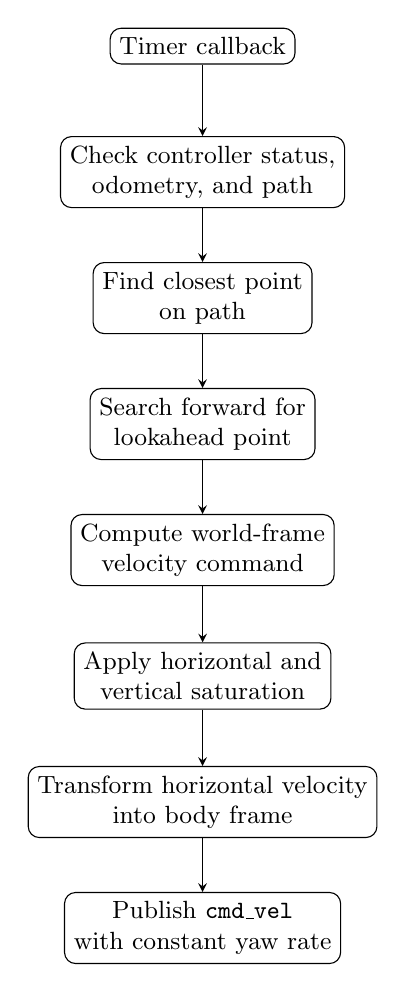
\begin{tikzpicture}[node distance=1.6cm, >=stealth, every node/.style={font=\small}]
\node[draw, rounded corners, align=center] (start) {Timer callback};
\node[draw, rounded corners, below of=start, align=center] (check1) {Check controller status,\\ odometry, and path};
\node[draw, rounded corners, below of=check1, align=center] (closest) {Find closest point\\ on path};
\node[draw, rounded corners, below of=closest, align=center] (lookahead) {Search forward for\\ lookahead point};
\node[draw, rounded corners, below of=lookahead, align=center] (control) {Compute world-frame\\ velocity command};
\node[draw, rounded corners, below of=control, align=center] (limit) {Apply horizontal and\\ vertical saturation};
\node[draw, rounded corners, below of=limit, align=center] (rotate) {Transform horizontal velocity\\ into body frame};
\node[draw, rounded corners, below of=rotate, align=center] (publish) {Publish \texttt{cmd\_vel}\\ with constant yaw rate};

\draw[->] (start) -- (check1);
\draw[->] (check1) -- (closest);
\draw[->] (closest) -- (lookahead);
\draw[->] (lookahead) -- (control);
\draw[->] (control) -- (limit);
\draw[->] (limit) -- (rotate);
\draw[->] (rotate) -- (publish);
\end{tikzpicture}
\caption{Overall flow of the controller. At each timer callback, the controller checks whether valid odometry and path data are available, selects a lookahead point, computes the translational velocity command, applies velocity limits, transforms the command into the body frame, and publishes the final control input.}
\label{fig:controller_flow}
\end{figure}


\subsection{Analysis of the Existing Algorithm}

The controller is designed to be simple and easy to implement. This is reasonable for the current project because the main requirement is reliable path following in simulation rather than high-performance flight control.

One advantage of the current design is that it is straightforward. The controller only depends on odometry and the planned path, and the logic is relatively easy to debug. This is useful in a course project, since it reduces implementation complexity and makes it easier to identify problems in either the planner, controller, or estimator.

Another advantage is that the use of a lookahead point gives smoother motion than directly commanding the drone toward the final goal at every time step. Instead of reacting only to the endpoint, the drone is guided along the path progressively. This makes the motion more natural and generally improves path tracking.

The explicit velocity limits are also important. By constraining horizontal and vertical motion separately, the controller satisfies the project requirements and avoids overly aggressive commands. This is especially useful for altitude control, where excessive vertical motion tends to cause more visible oscillation.

However, the controller also has some limitations. First, the lookahead distance is fixed. This means the same value is used for straight motion, turning, and final approach. In practice, a larger lookahead usually gives smoother motion but tends to cut corners, while a smaller lookahead improves path accuracy but can lead to sharper corrections.

Second, the controller uses only proportional feedback based on position error. It does not explicitly account for the drone's current velocity, and it does not predict future motion. As a result, the response may not be as smooth as a more advanced controller, particularly when the drone is close to the target.

Third, the closest path point is chosen based only on Euclidean distance. This works well enough for short and simple paths, but it may become less reliable if the drone deviates significantly from the path or if the path shape becomes more complicated.

Finally, the yaw motion is fully separated from translational path following. This is acceptable here because the yaw rate is specified as a fixed requirement, but it means the controller does not actively choose an orientation that helps tracking performance.

Overall, the current controller is a reasonable baseline solution. It is simple, functional, and suitable for the scope of the project, although it is not intended to be a highly refined tracking controller.

\subsection{Justification of Parameter Choices}

The main parameters in the controller are the lookahead distance, maximum horizontal velocity, maximum vertical velocity, yaw velocity, and the proportional gains for horizontal and vertical motion.

The lookahead distance determines how far ahead on the path the controller tries to follow. If the value is too small, the drone may react too strongly to small path changes or estimation noise. If the value is too large, the drone may cut corners and become less accurate when approaching waypoints. For this reason, a moderate lookahead distance is more suitable.

The maximum horizontal and vertical velocities are chosen according to the project constraints. These limits are important because they directly affect the safety and smoothness of the motion. In particular, the vertical velocity limit should remain relatively small, since altitude changes are usually more sensitive and more likely to oscillate.

The proportional gain in the horizontal plane should be high enough for the drone to respond promptly to the path, but not so high that it produces unstable or oscillatory motion. Similarly, the vertical gain should be chosen more conservatively, since vertical motion is more likely to overshoot when the gain is too large.

The yaw velocity must also be chosen carefully, since the project specifies a constant clockwise rotation rate. Because ROS uses radians per second, the desired angular speed must be converted correctly from degrees per second.

\subsection{Possible Improvements}

Although the current controller works reasonably well, several simple improvements could make it perform better without changing the overall structure too much.

One possible improvement is to use an adaptive lookahead distance. For example, the controller could use a larger lookahead when the drone is far from the goal and a smaller lookahead when it is close to a waypoint. This would help balance smooth motion and tracking accuracy.

Another possible improvement is to reduce the commanded speed more deliberately when the drone is near the final target. While proportional control already decreases the velocity as the position error becomes smaller, an additional speed scheduling rule could make the final approach smoother.

A third improvement is to keep track of the previously selected closest path index and continue searching from there, instead of searching the full path every time. This would reduce the chance of the controller jumping backward to an earlier point on the path.

A small deadband around the target position or target altitude could also help. Once the drone is sufficiently close to the desired point, very small corrections may not be necessary and may only introduce visible jitter due to noise.

These improvements are relatively simple and can be added without replacing the basic controller design.

\subsection{Discussion}

From a practical point of view, the current controller achieves a good balance between simplicity and functionality. It satisfies the main project requirements, namely path following, velocity limiting, and constant yaw rotation. It is also easy to understand and implement, which is important in a course project where the emphasis is not only on performance but also on correctness and clarity.

At the same time, the controller still behaves like a basic proportional path follower. It does not adapt itself to different path geometries, and it does not explicitly optimize tracking accuracy or smoothness. Therefore, while it is sufficient for the current simulation task, it should be seen as a simple baseline rather than a complete flight control solution.

\subsection{Summary}

In summary, the controller uses a lookahead-based path-following method that suits a holonomic drone well. The implementation is straightforward, respects the required motion constraints, and is sufficient for the project task. Its main strengths are simplicity and ease of tuning, while its main weaknesses are the use of a fixed lookahead distance and a basic proportional control law. Even so, the controller provides a practical and effective solution for this project.

\section{Estimator}

\subsection{Algorithm Examination}

The handout already gives the basic filter structure, so here we only keep the parts needed to explain our final implementation and our changes.

\subsubsection{State Decomposition}

We keep the axis-by-axis structure from the handout. Instead of one large coupled filter, we use four small filters:
\[
    X_x = [x,\, v_x]^T,\quad
    X_y = [y,\, v_y]^T,\quad
    X_z = [z,\, v_z,\, b_{\text{baro}}]^T,\quad
    X_a = [\psi,\, \dot{\psi}]^T
\]
where $b_{\text{baro}}$ is the barometer bias and $\psi$ is yaw. This is still a simple estimator, not a full 3D EKF.

\subsubsection{Prediction Step}

The IMU callback performs the prediction step. Let $(u_x, u_y, u_z)$ be the linear acceleration from the IMU in the drone frame. We rotate the horizontal acceleration into the world frame using the current yaw:
\[
    a_x = \cos \psi \, u_x - \sin \psi \, u_y,\qquad
    a_y = \sin \psi \, u_x + \cos \psi \, u_y
\]
Then the $x$ and $y$ filters use a constant-acceleration model:
\[
    \begin{aligned}
        x_{k+1} &= x_k + v_{x,k}\Delta t + \frac{1}{2} a_x \Delta t^2 \\
        v_{x,k+1} &= v_{x,k} + a_x \Delta t
    \end{aligned}
\]
The same form is used for $y$.

For the vertical axis, we first remove gravity:
\[
    a_z = u_z - g
\]
In the code, $a_z$ is also clamped to $\pm 1.5\,\text{m/s}^2$ to limit IMU spikes. The $z$ state is predicted by
\[
    \begin{aligned}
        z_{k+1} &= z_k + v_{z,k}\Delta t + \frac{1}{2} a_z \Delta t^2 \\
        v_{z,k+1} &= v_{z,k} + a_z \Delta t \\
        b_{\text{baro},k+1} &= b_{\text{baro},k}
    \end{aligned}
\]
Yaw is predicted from the IMU angular velocity:
\[
    \psi_{k+1} = \psi_k + \omega_z \Delta t
\]
and the angle is wrapped after each update.

\subsubsection{Correction Models}

The correction step is also separated by sensor. Table~\ref{tab:estimator_measurements} shows the measurement models used in the final code.

\begin{table}[!t]
    \centering
    \small
    \setlength{\tabcolsep}{6pt}
    \caption{Measurement models used by the estimator.}
    \label{tab:estimator_measurements}
    \vspace{0.1cm}
    \begin{tabular}{llll}
        \toprule
        \textbf{Sensor} & \textbf{Measurement} & \textbf{Model} & \textbf{Updated state} \\
        \midrule
        GPS & position & $z_{\text{gps}} = [x,\, y,\, z]^T$ & $X_x$, $X_y$, $X_z$ \\
        Sonar & height & $z_{\text{sonar}} = z$ & $X_z$ \\
        Barometer & altitude & $z_{\text{baro}} = z + b_{\text{baro}}$ & $X_z$ \\
        Magnetometer & yaw & $z_{\text{mag}} = \psi$ & $X_a$ \\
        \bottomrule
    \end{tabular}
\end{table}

The first GPS message initializes the local origin. After that, GPS measurements are converted from latitude, longitude, and altitude into ECEF, then into a local NED frame, and finally into Gazebo's ENU map frame. The magnetometer yaw is computed by
\[
    \psi_{\text{mag}} = \text{atan2}(-m_y,\, m_x)
\]
The barometer altitude is computed from pressure by
\[
    z_{\text{baro}} = 44330 \left(1 - \left(\frac{P}{101325}\right)^{0.1903}\right)
\]

For scalar corrections, we update the covariance with the Joseph form:
\[
    P^+ = (I - KH)P^-(I - KH)^T + KRK^T
\]
We keep this form for numerical stability.

\subsection{Improvements}

\subsubsection{Sonar Gating}

In our early runs, the sonar helped near the ground but became unreliable higher up. In the final code, we only accept the sonar update when the predicted height is at most $3.8\,\text{m}$ and the innovation is at most $1.0\,\text{m}$.

\subsubsection{Barometer Bias State}

We observed a noticeable barometer offset. Treating it as a direct measurement of $z$ gave a biased height estimate. In the final version, we add a bias term $b_{\text{baro}}$ into the vertical state and use
\[
    H_{\text{baro}} = [1 \;\; 0 \;\; 1]
\]
The first barometer message initializes the bias by $b_{\text{baro}} = z_{\text{baro}} - z$. After that, the filter can absorb the slow offset into the bias state instead of pushing it into the altitude estimate.

\subsubsection{GPS Velocity Correction}

Our main problem in the horizontal plane was lag. The estimate was usually stable, but it tended to stay behind the true motion. To reduce this, the estimator computes a planar pseudo-velocity from two consecutive GPS positions:
\[
    \hat{v}_{\text{gps}} = \frac{p_k - p_{k-1}}{\Delta t}
\]
This velocity is smoothed and then used as a correction for $v_x$ and $v_y$. We keep this update conservative. It is only used when the GPS time gap is reasonable and when the velocity innovation is not too large.

\subsubsection{GPS Forward Compensation}

GPS messages may arrive slightly later than the latest predicted state. If we correct with an old GPS position directly, the estimate stays behind the true motion. To reduce this mismatch, we forward-compensate the GPS position using the current estimated velocity:
\[
    p_{\text{gps,corr}} = p_{\text{gps}} + \hat{v}\,\Delta t_{\text{lag}}
\]
This correction is only applied when the lag is positive and smaller than $0.5\,\text{s}$.

\subsection{Parameter Tuning}

Table~\ref{tab:estimator_params} lists the main estimator parameters used in the final submission. We only include the parameters that directly affect the final behavior. The final values were chosen to improve the observed height error and horizontal lag, not to copy one lucky run.

We based this on several small parameter sweeps and repeat runs, and kept values that stayed stable across runs instead of the single best number from one trial.

\begin{table}[!t]
    \centering
    \small
    \caption{Main estimator parameters.}
    \label{tab:estimator_params}
    \vspace{0.1cm}
    \resizebox{0.95\linewidth}{!}{%
    \begin{tabular}{lll}
        \toprule
        \textbf{Parameter} & \textbf{Value} & \textbf{Reason} \\
        \midrule
        \texttt{frequency} & $30.0$ Hz & Faster odom updates \\
        \texttt{var\_imu\_x}, \texttt{var\_imu\_y} & $1.5$ & Stable horizontal tuning \\
        \texttt{var\_imu\_z} & $20.0$ & Reduce trust in vertical IMU prediction \\
        \texttt{var\_gps\_x}, \texttt{var\_gps\_y} & $0.15$ & Reduce $x/y$ lag \\
        \texttt{var\_gps\_z} & $0.5$ & GPS height is secondary \\
        \texttt{var\_sonar} & $0.03$ & Strong low-altitude correction \\
        \texttt{var\_baro} & $1.0$ & Moderate barometer trust \\
        \texttt{gps\_forward\_compensation\_max\_dt} & $0.5$ s & Limit stale GPS compensation \\
        \texttt{gps\_velocity\_alpha} & $0.9$ & Smooth GPS pseudo-velocity \\
        \texttt{gps\_velocity\_variance\_scale} & $0.1$ & Keep velocity correction light \\
        \texttt{gps\_velocity\_min\_variance} & $0.04$ & Avoid over-trusting pseudo-velocity \\
        \texttt{gps\_velocity\_max\_innovation} & $1.5$ & Reject inconsistent velocity updates \\
        \bottomrule
    \end{tabular}%
    }
\end{table}

Our tuning logic is simple. The $z$ axis is mainly stabilized by sonar gating and the barometer bias state, so we keep the vertical IMU variance large. The largest remaining error is still in $x$ and $y$, so we keep the GPS position variance smaller and leave the pseudo-velocity correction enabled.

\subsection{Representative Comparison}

Table~\ref{tab:estimator_before_after} shows a before-and-after comparison for the $z$ axis. The baseline comes from an early 40-second sweep, and the improved result comes after the $z$-axis fixes. We use this table to show that the main height failure was removed.

\begin{table}[!t]
    \centering
    \small
    \setlength{\tabcolsep}{8pt}
    \caption{Representative before-and-after comparison for the $z$ axis.}
    \label{tab:estimator_before_after}
    \vspace{0.1cm}
    \begin{tabular}{lcc}
        \toprule
        \textbf{Case} & \textbf{All-data $z$ MAE} & \textbf{$7$--$25$ s $z$ MAE} \\
        \midrule
        Early baseline & $0.649$ m & $0.533$ m \\
        After $z$-axis fixes & $0.020$ m & $0.019$ m \\
        Repeat run after fixes & --- & $0.020$ m \\
        \bottomrule
    \end{tabular}
\end{table}

This comparison supports our main claim for the vertical axis. The main change is in the sensor model: unreliable high-altitude sonar updates are rejected, and barometer bias is estimated as a state.

Figure~\ref{fig:estimator_z_before_after} shows the same comparison visually. In the early baseline, the estimated height drops far below the true value several times after about $16$ s. After the $z$-axis fixes, the height trace stays close to ground truth.

\begin{figure}[!tbp]
    \centering
    \begin{minipage}[t]{0.49\linewidth}
        \centering
        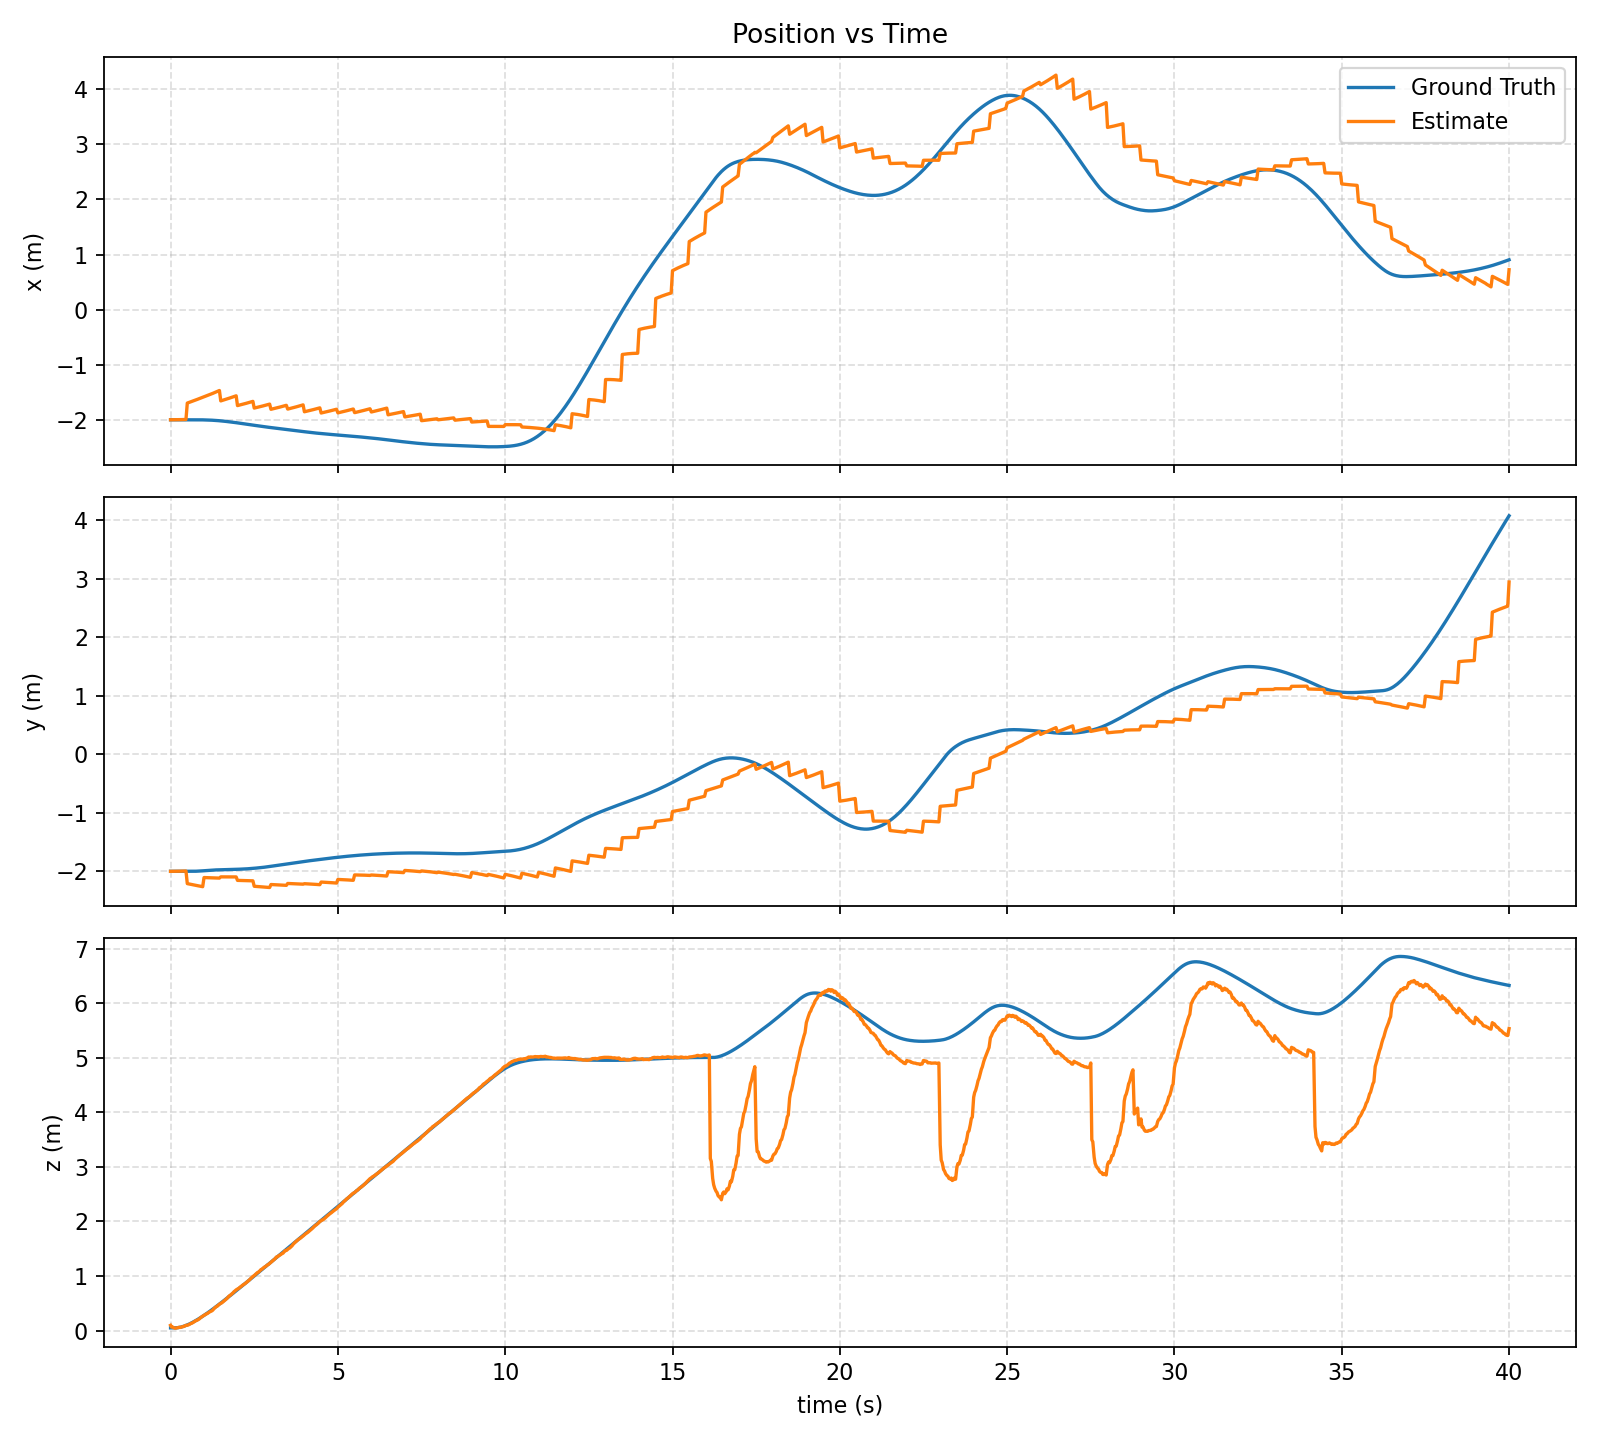
\includegraphics[width=\linewidth]{figures/estimator_z_baseline_position.png}
    \end{minipage}\hfill
    \begin{minipage}[t]{0.49\linewidth}
        \centering
        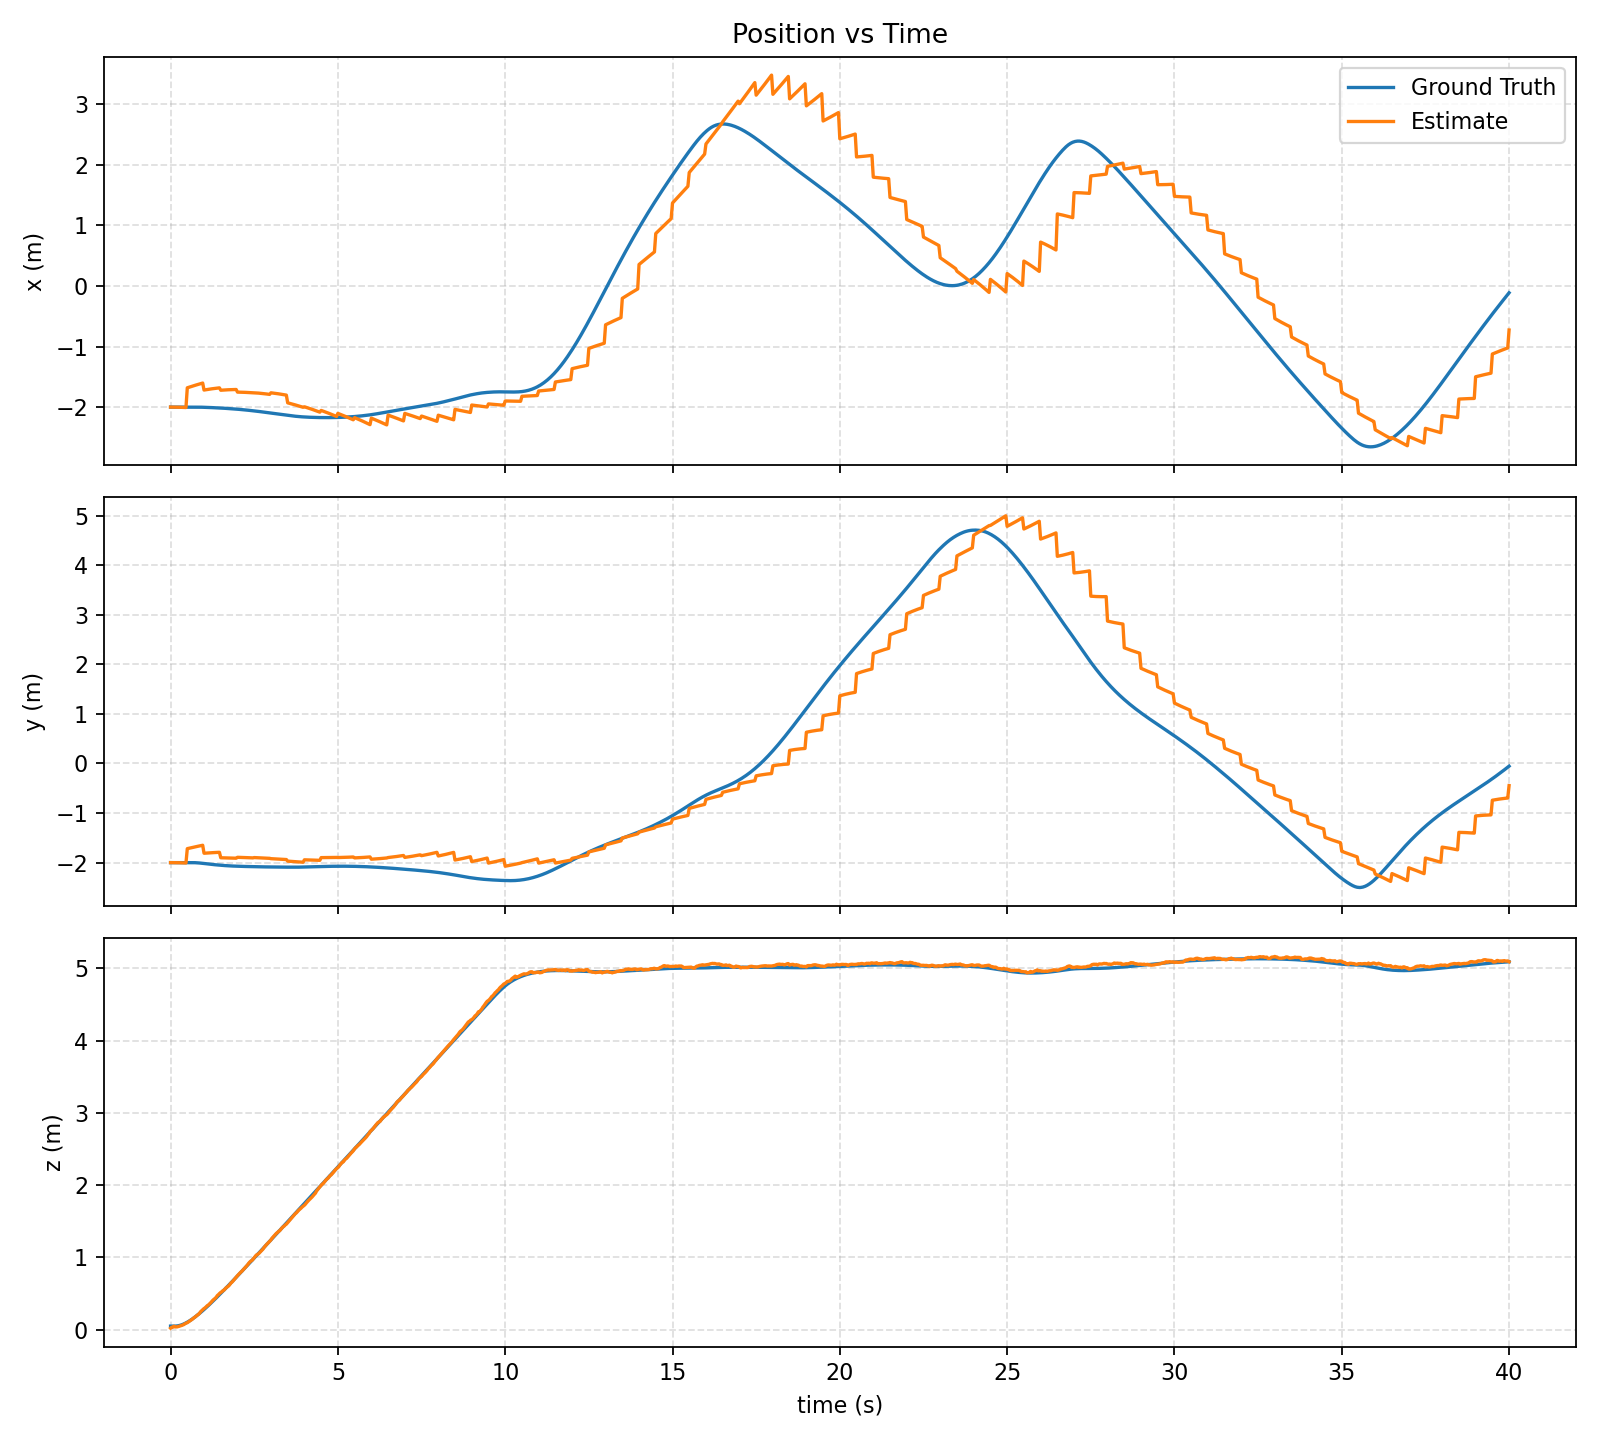
\includegraphics[width=\linewidth]{figures/estimator_z_fixed_position.png}
    \end{minipage}
    \caption{Representative position traces before and after the $z$-axis fixes. Left: early baseline, where the estimated height becomes unreliable in the second half of the run. Right: after sonar gating and barometer bias augmentation, where the $z$ estimate remains close to ground truth.}
    \label{fig:estimator_z_before_after}
\end{figure}

\subsection{Final Performance}

Table~\ref{tab:estimator_results} shows the result of the final validation experiment. The main conclusion is that the $z$ and yaw estimates are already quite accurate, while $x$ and $y$ are still the main limitation.

\begin{table}[!t]
    \centering
    \small
    \setlength{\tabcolsep}{10pt}
    \caption{Final validation result.}
    \label{tab:estimator_results}
    \vspace{0.1cm}
    \begin{tabular}{lcccc}
        \toprule
        \textbf{Metric} & \textbf{$x$} & \textbf{$y$} & \textbf{$z$} & \textbf{yaw} \\
        \midrule
        MAE & $0.2099$ m & $0.3018$ m & $0.0199$ m & $0.00435$ rad \\
        RMSE & $0.2877$ m & $0.3832$ m & $0.0256$ m & $0.00551$ rad \\
        \bottomrule
    \end{tabular}
\end{table}

These results match what we observed during testing. The vertical estimate is good because sonar and barometer help in different ways, and the yaw estimate is also accurate because the magnetometer gives a direct heading correction. The main remaining weakness is horizontal lag, but the estimator is still stable enough for the full mission.

\begin{figure}[!tbp]
    \centering
    \begin{minipage}[t]{0.48\linewidth}
        \centering
        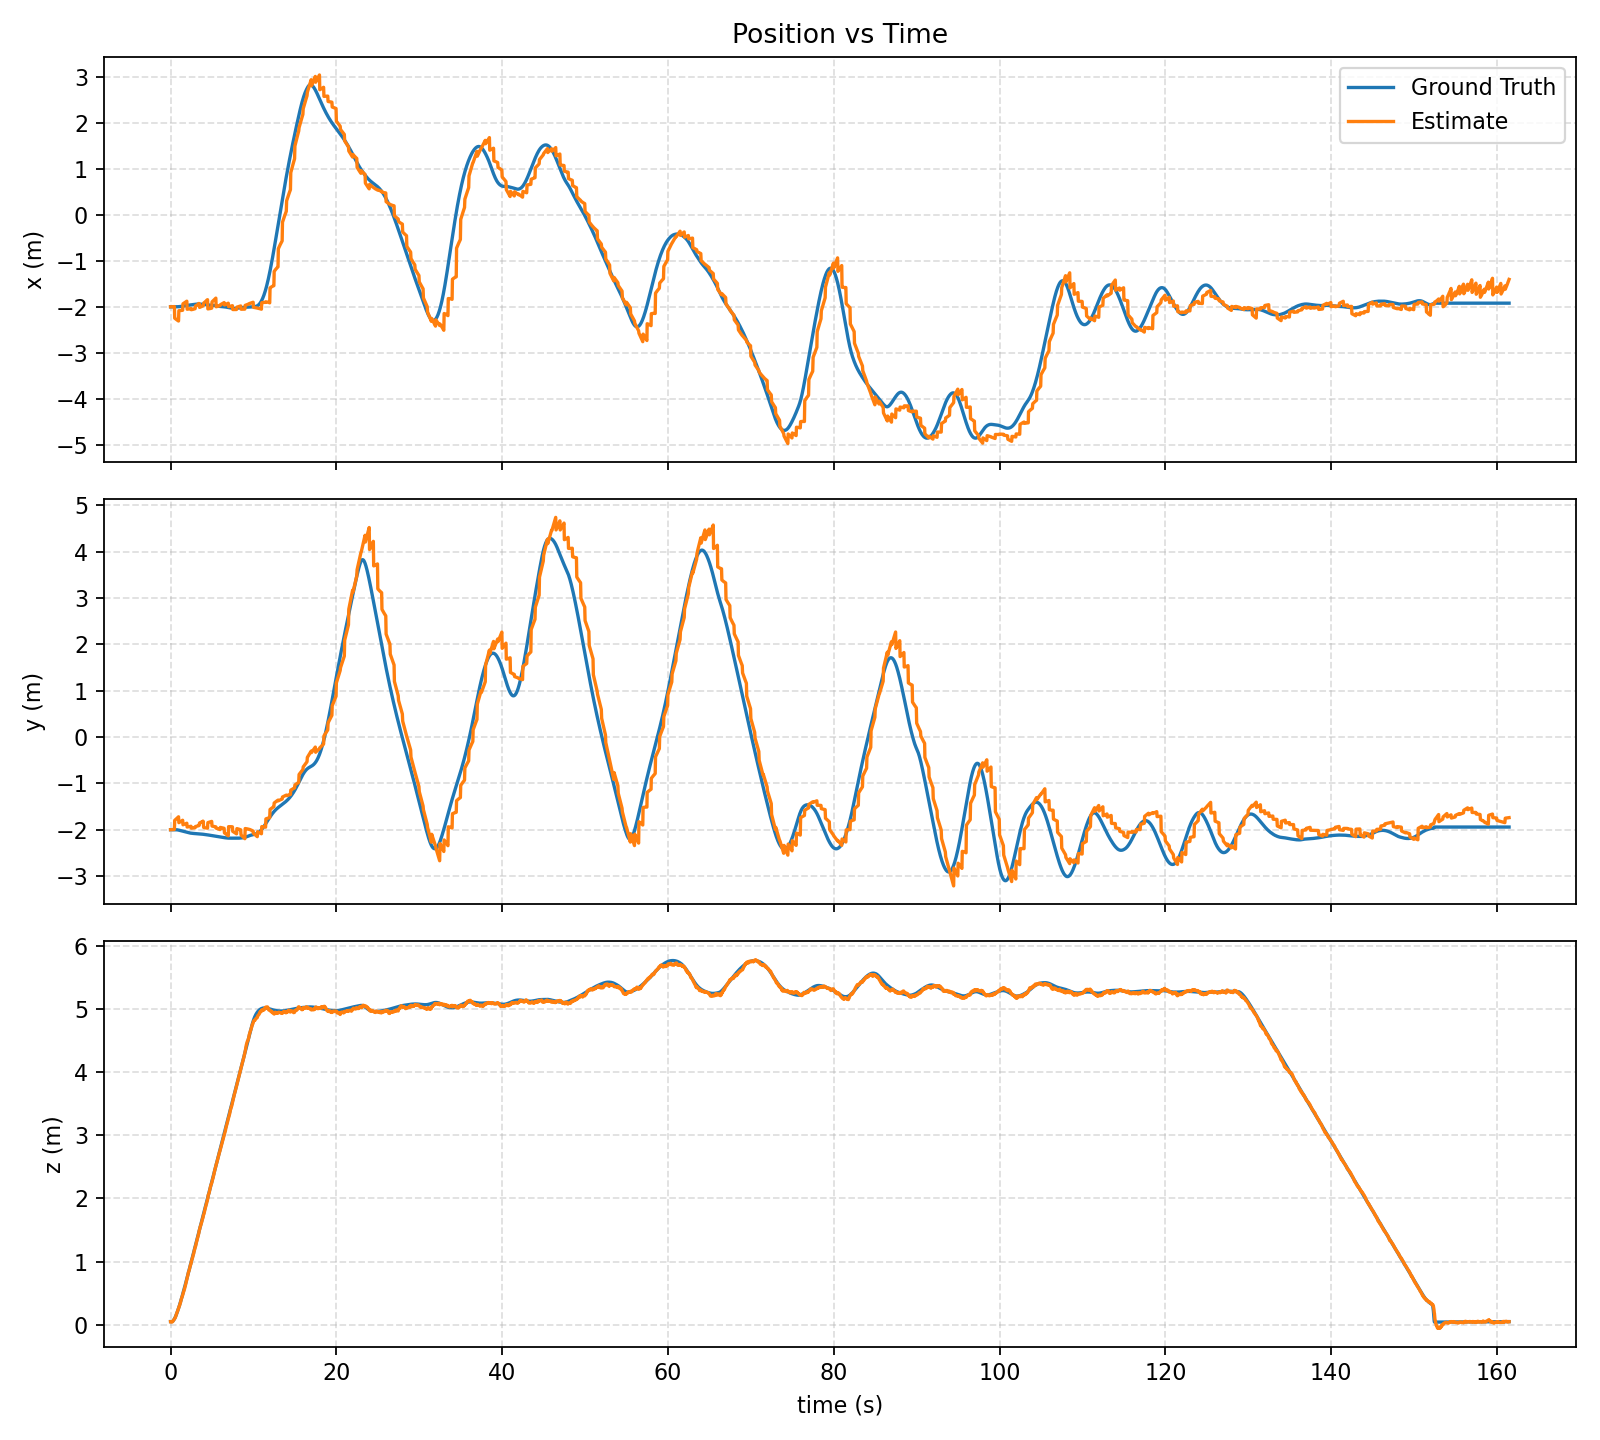
\includegraphics[width=\linewidth]{figures/estimator_position_vs_time.png}
    \end{minipage}\hfill
    \begin{minipage}[t]{0.48\linewidth}
        \centering
        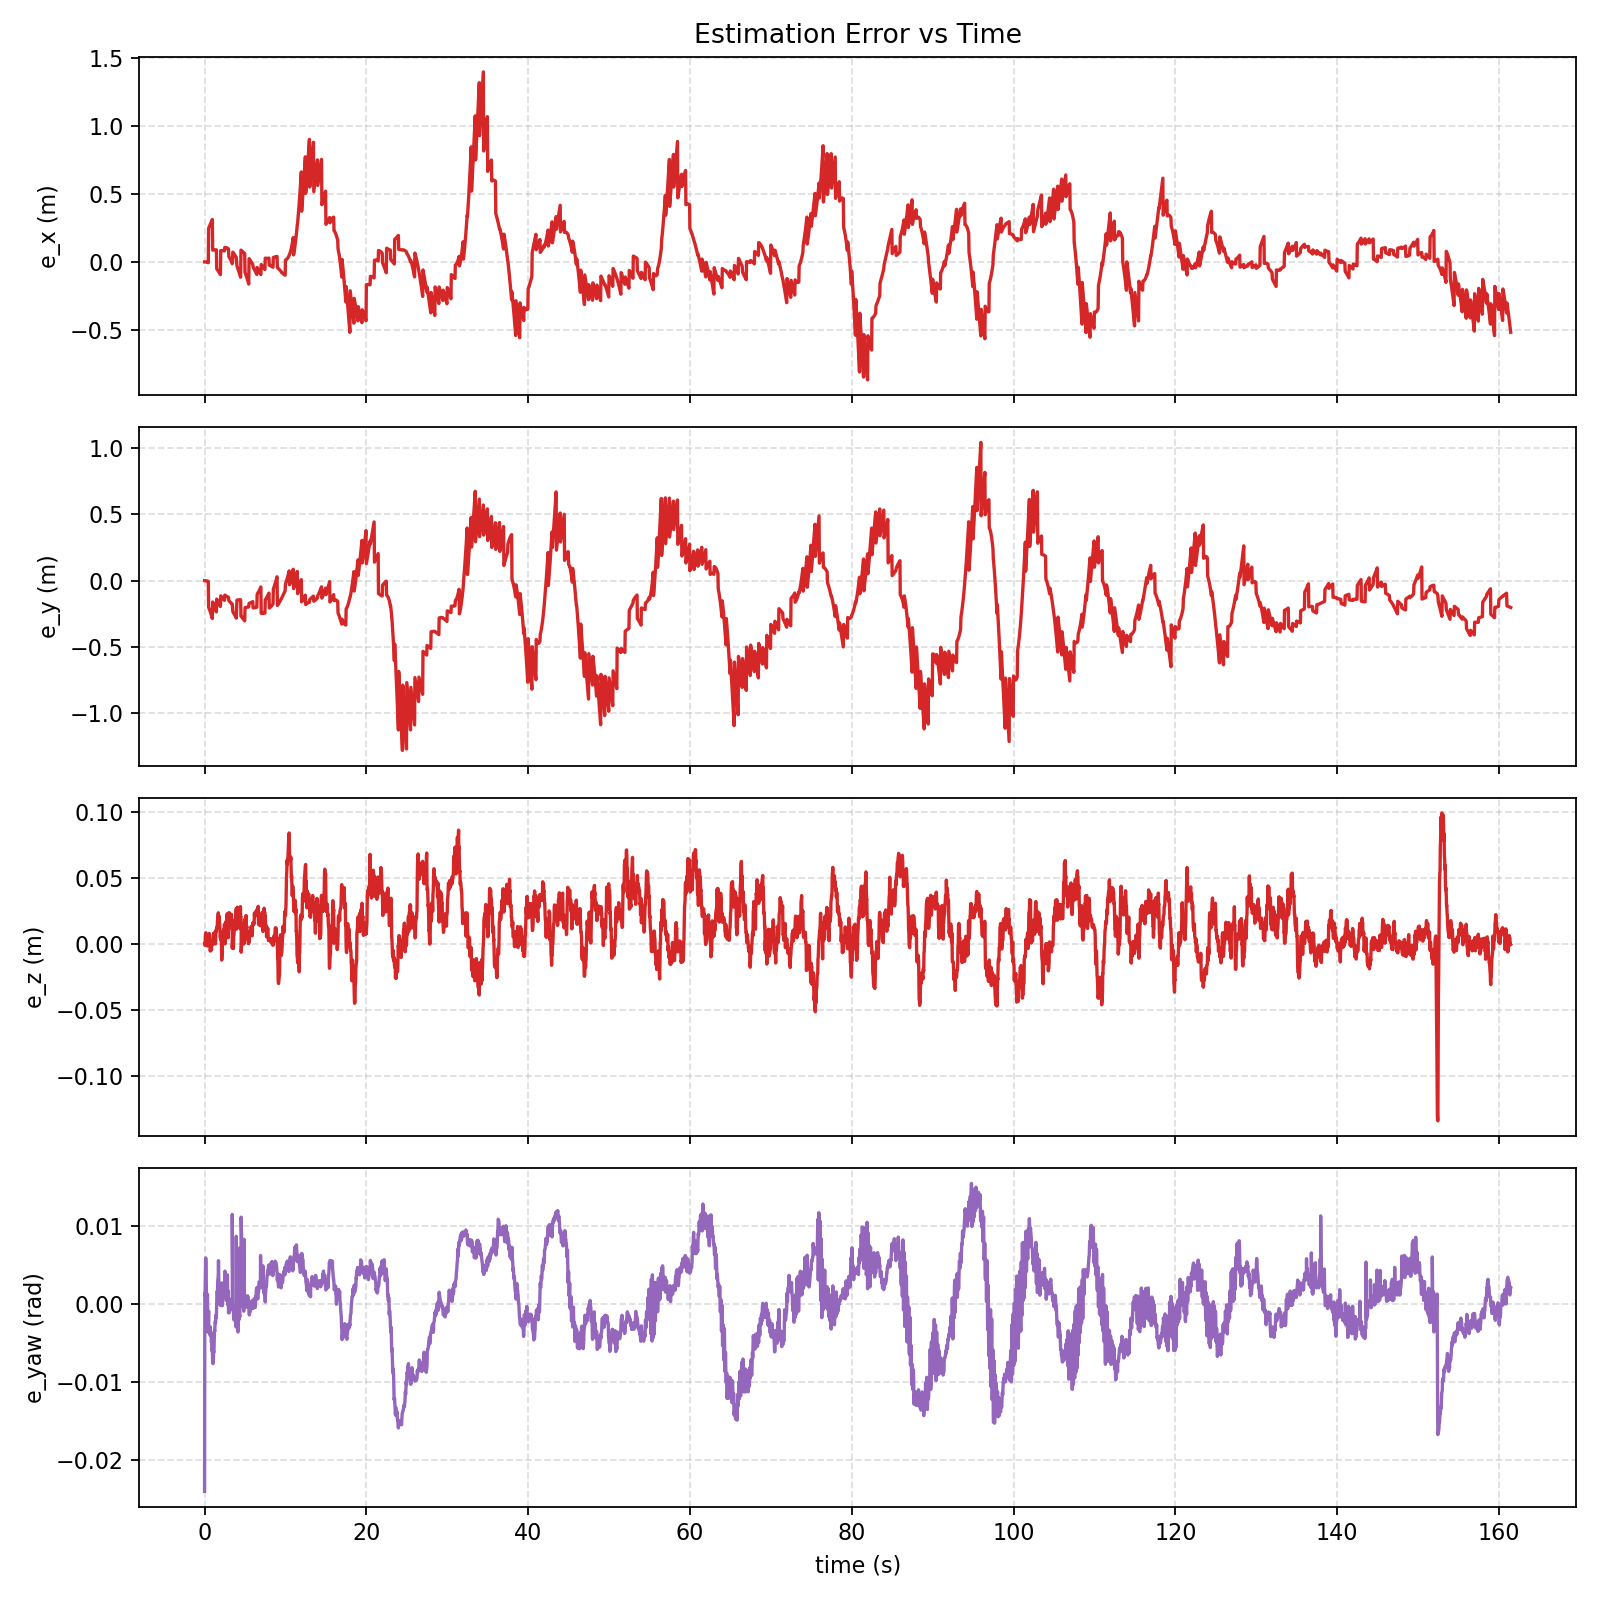
\includegraphics[width=\linewidth]{figures/estimator_error_vs_time.png}
    \end{minipage}
    \caption{Left: position traces in the final validation experiment. The $z$ estimate stays close to ground truth during takeoff, cruise, and landing, while the larger visible mismatch remains in the horizontal axes. Right: estimation error in the final validation experiment. The $z$ and yaw errors remain small throughout the mission, while the larger residual oscillations are concentrated in $x$ and $y$.}
    \label{fig:estimator_final_results}
\end{figure}

\section{Contribution}

\begin{itemize}
    \item \textbf{A0319170J:} Implemented the behavior node, including the seven-state FSM design, live waypoint tracking for the \textsc{Turtle\_Position} state, cycle-completion guarantee, and path availability guard. Tuned all behavior node parameters. Contributed to the report (Section~1: Behavior).
    \item \textbf{A0318793N:} Implemented the path-following controller, including lookahead point selection, proportional velocity control, velocity saturation, world-to-body frame transformation, and constant yaw rate command. Tuned all controller parameters. Contributed to the report (Section~2: Controller).
    \item \textbf{A0326802J:} Implemented the Kalman filter estimator, including state decomposition, IMU prediction, multi-sensor correction models, sonar gating, barometer bias state, GPS velocity correction, and GPS forward compensation. Tuned all estimator parameters. Contributed to the report (Section~3: Estimator).
    \item All three members jointly integrated and debugged the full drone mission stack in simulation, participated in code review, and contributed to the writing and proofreading of the report.
\end{itemize}

\section{AI Tool Declaration}
We used Sonnet 4.6 during the completion of this project.

\end{document}
